\documentclass[a4paper, 10pt, fleqn]{article}

\usepackage[utf8]{inputenc}
\usepackage[T1]{fontenc}
\usepackage{textcomp}
\usepackage{lmodern}
\usepackage[ngerman]{babel}
\usepackage{tocbibind}
\usepackage{enumerate}
%\usepackage{xcolor}
\usepackage[table]{xcolor}
\usepackage{pdfpages}
\usepackage{amsmath}
\usepackage{graphicx}
\usepackage{geometry}
\usepackage{scrpage2}
\usepackage{lastpage}
\usepackage[hyphens]{url}
\usepackage{hyperref}
\usepackage{listings}
\usepackage{float}
\restylefloat{figure}
\lstset{language=[ansi]C++}

\newcommand{\code}[1]{\texttt{#1}}

\renewcommand*{\listoffigures}{%
  \begingroup
  \tocchapter
  \tocfile{\listfigurename}{lof}
  \endgroup
}

\geometry{left=3cm, top=3cm, bottom=3cm, right=2cm}

\hypersetup{
    colorlinks,
    linkcolor=black,
    citecolor=black,
    urlcolor=black
}

\pagestyle{scrheadings}
\ihead{APPE Team 13}\ohead{Projektmanagementplan}
\ifoot{\today} \ofoot{Seite \thepage\ von {\hypersetup{linkcolor=black}\pageref{LastPage}}}

% Einrücken zu Beginn von neuem Absatz unterdrücken
\setlength{\parindent}{0pt}

% Zeilenabstand einstellen
\usepackage{setspace}
\makeatletter
\newcommand{\MSonehalfspacing}{%
  \setstretch{1.44}%  default
  \ifcase \@ptsize \relax % 10pt
    \setstretch {1.448}%
  \or % 11pt
    \setstretch {1.399}%
  \or % 12pt
    \setstretch {1.433}%
  \fi
}
\newcommand{\MSdoublespacing}{%
  \setstretch {1.92}%  default
  \ifcase \@ptsize \relax % 10pt
    \setstretch {1.936}%
  \or % 11pt
    \setstretch {1.866}%
  \or % 12pt
    \setstretch {1.902}%
  \fi
}
\makeatother
\MSonehalfspacing

\begin{document}
%Zweifarbige Tabellen als Standard
\rowcolors{2}{gray!25}{white}
%
% !TEX root = Dokumentation.tex
\begin{titlepage}   

\begin{center}
\textsc{\Large Team 13}\\[0.5cm]

% Title
\newcommand{\HRule}{\rule{\linewidth}{0.5mm}}
\HRule \\[0.4cm]
{ \huge \bfseries Filialbestellsystem}\\[0.4cm]
{ \LARGE \bfseries Projektmanagementplan}\\[0.4cm]
\HRule \\[1.5cm]

% Unterer Teil der Seite
{\large Rotkreuz, \today}

\begin{figure}[H]%Position festigen
\centering
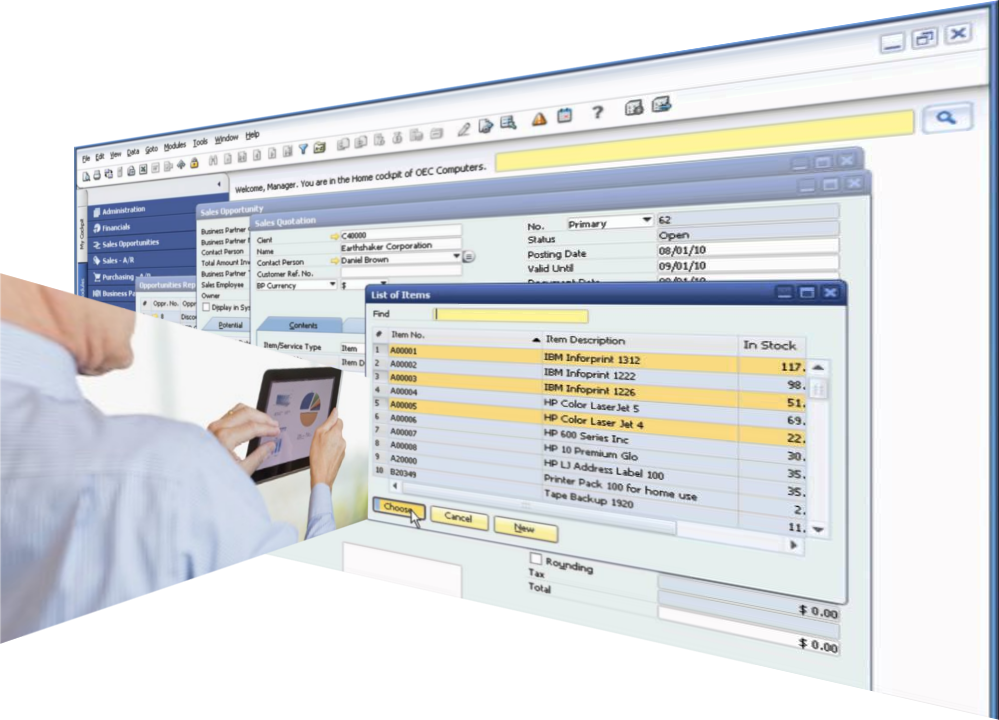
\includegraphics[width=0.7\textwidth]{Images/Titelbild.png}
\label{fig:title}
\end{figure}
% Author and supervisor
\begin{minipage}{0.4\textwidth}
\begin{flushleft} \large
\emph{Autoren:}\\
Marco Moro\\
Severin Gmür\\
Ramon Wyss\\
Tobias Kreienbühl\\
\end{flushleft}
\end{minipage}
\hfill
\begin{minipage}{0.4\textwidth}
\begin{flushright} \large
%\emph{Supervisor:} \\
%tbd
\end{flushright}
\end{minipage}
\large
\vfill
I.BA\_APPE.F1701 \\
Hochschule Luzern Informatik

\end{center}

\end{titlepage}
\tableofcontents
\clearpage
% !TEX root = Dokumentation.tex
\section{Projektüberblick}
Das folgende Kapitel definiert die organisatorischen Aspekte im Zusammenhang mit dem Entwicklungsprojekt in APPE. Es umfasst dabei die Projektziele \&-resultate.
\subsection{Projektauftrag, Ziele \& Resultate}
Der Kunde hat ein Informatik-System für ein elektronisches Artikel-Bestellsystem für seine dezentralen Filialen bestellt.\\
Jede Filiale hat ein lokales Lager, welches in einer lokalen Datenbank (pro Filiale) verwaltet wird. Daneben existiert auch ein zentrales Lager, dieses wird in einem bestehenden System (Legacy System) verwaltet, welches über eine zur Verfügung gestellte Komponente einzubinden ist. Im zentralen Lager sind die Artikel entweder sofort lieferbar oder müssen nachbestellt werden.
\subsubsection{Ziele}
Mit dem Projekt sind dabei folgende Ziele zu erreichen:\\
\textbf{Funktionale Ziele / Anforderungen}
\begin{itemize}
\item Das Verkaufspersonal kann per Telefon, Schalterkontakt, Fax oder Mail eingegangene Bestellungen im System erfassen, d.h. es können Artikel aus einem Katalog auswählt, die Verfügbarkeit der Artikel geprüft und die Bestellung ausgeführt werden.
\item Auch wenn mehrere Benutzer einer Filiale gleichzeitig im System arbeiten, dürfen keine inkonsistenten Zustände entstehen (Bsp.: gleiches Exemplar mehrfach verkaufen)
\item Benutzer/innen des Systems müssen sich mit Name und Passwort identifizieren, ihnen werden danach entsprechende Rechte zugeteilt. (Benutzergruppen: SysAdmin, Filialleiter/in, Verkäufer/in, Datentypist/in)
\item Der Filialverwalter kann die Vorgänge im System (Fehler, wesentliche Geschäftsvorfälle) anhand von Logbucheinträgen laufend überwachen.
\item Der Filialleiter kann jederzeit die aktuellen Bestellungen, Nachbestellungen und Lieferungen aus der Zentrale einsehen
\item Der/die Datentypist/in kann im System angelieferte Artikel im Filiallager eintragen.
\item Das Verkaufspersonal und der Filialleiter können jederzeit den Zustand der Bestellungen einsehen. Eine Bestellung kann auch geändert oder annulliert werden.
\item Jegliche Exception und pro wesentlicher Business-Vorgang werden Logger-Einträge mitteils einem Logging-Framework aufgezeichnet.
\end{itemize}

\textbf{Organisatorische Ziele / Anforderungen}
\begin{itemize}
\item Alle Gruppenmitglieder müssen in der Softwareerstellung involviert sein. Die entsprechenden Verantwortlichkeiten sind in der Dokumentation ausgewiesen.
\end{itemize}

\textbf{Abgrenzungen \& Vorgaben}
\begin{itemize}
\item Die Buchhaltung inkl. Mahnwesen für die Rechnungsstellung/-behandlung erfolgt in einer separaten RW-Applikation mit Zugriff auf die lokale DB und ist nicht Teil des Auftrages.
\item Der Datenbankserver wird zur Verfügung gestellt.
\item Die Komponente für die Einbindung des Legacy Systems (Zentrallager) wird durch den Auftraggeber geliefert / zur Verfügung gestellt.
\end{itemize}

\subsubsection{Resultate}
Im Bereich der Softwareentwicklung sind entsprechende Resultate auszuweisen. Dabei werden in der Systemspezifikationen folgende Resultate beschrieben:
\begin{itemize}
\item Ein Kontext-Diagramm
\item Übersichtsdiagramm aller Use Cases inkl. einer Kurzbeschreibung der Use Cases. Detaillierte Beschreibung des Use Cases 'Bestellung ausführen'.
\item Konzeptionelles Datenmodell
\item Architektur-Modell(e) und nachvollziehbare Architekturentscheide
\item Schnittstellen-Spezifikation(en)
\end{itemize}

Im PMP werden dabei folgende Resultate abgebildet:
\begin{itemize}
\item Projektverantwortlichkeiten
\item Rahmenplan mit wichtigen Meilensteinen und Sprints
\item Dokumentation der Epics und Stories inkl. der Akzeptanzkriterien.
\item Testplan \& Testprotokoll
\end{itemize}

Auf applikatorischer Ebene werden folgende Softwaredeliverables erwartet:\\
Ein lauffähiges Programm, welches:
\begin{itemize}
\item in der vorgegebenen Projektstruktur auf GitLab verwaltet wird.
\item über einen automatisierten Build verfügt und auf dem Buildserver laufend integriert wird (CI)
\item automatisierte (Unit-)Tests ohne Fehler durchläuft und über eine begründete minimale Codeabdeckung verfügt
\end{itemize}

\subsection{Organisation, Rollen \& Zuständigkeiten}
Das Projektteam besteht aus vier Personen. Aufgrund dieser geringen Anzahl wird grundsätzlich keine hierarchische Organisationsform angestrebt. Primär werden Lösungen und Entscheidung mit einem gemeinsamen Konsens gefunden / gefällt. Bei unentschiedener Ausgangslage entscheidet der Projektleiter endgültig.
Die Rollen und Zuständigkeiten definieren die u.a. die Aufgaben und Verantwortungen einer Rolle und sind für unser Team wie folgt definiert:
% !TEX root = Dokumentation_PMP.tex
\begin{table}[H]
\begin{tabular}{ | p{0.22\textwidth} | p{0.19\textwidth} |  p{0.47\textwidth} |}
\hline \rowcolor{gray!50}
%Titelzeile
	\textbf{Rolle}          &
	\begin{tabular}{l}
		\textbf{Verantwortung}
	\end{tabular}	 	 &
	\begin{tabular}{l}
		\textbf{Aufgaben}
	\end{tabular}
	\\ \hline
%Zeile
	\textbf{Projektmanagement}			 &
	\begin{tabular}{l}
		Marco M.
	\end{tabular}	 	 			&
	\begin{tabular}{l}
		Ist für das Projektmanagement verantwortlich \\
		und führt Protokolle, Risikoliste und stellt \\
		bei Bedarf die externe Kommunikation sicher
	\end{tabular}
\\ \hline
%Zeile
	\textbf{Anforderungs-management}   		 &
	\begin{tabular}{l}
		Severin G.
	\end{tabular}	 	 			&
	\begin{tabular}{l}
		Klärt die funktionalen und nicht \\
		funktionalen Anforderungen ab
	\end{tabular}
\\ \hline
%Zeile
	\textbf{Dokument- \& Codeverwaltung}   		 &
	\begin{tabular}{l}
		Tobias K.
	\end{tabular}	 	 			&
	\begin{tabular}{l}
		Erstellung \& Verwaltung der Dokumentationen \\
		inkl. zentraler Ablage \& Versionierung \& \\
		Austausch Codesourcen mittels Git
	\end{tabular}
\\ \hline
%Zeile
	\textbf{Softwarearchitektur}              & 
	\begin{tabular}{l}
		Tobias K.
	\end{tabular}                 &
	\begin{tabular}{l}
		Plant und entwirft die SW-Architektur und \\
		definiert Schnittstellen. Prüft, ob die Archi-\\
		tektur (Layering, etc.) korrekt umgesetzt wurde
	\end{tabular}
\\ \hline
%Zeile
	\textbf{SW-Entwicklung Layer Data}       &
	\begin{tabular}{l}
		Ramon W.
	\end{tabular}	 	 &
	\begin{tabular}{l}
		Ist für die SW-Entwicklung des Layers Data \\
		verantwortlich und stellt dadurch die Daten-\\
		grundlage des Systems zur Verfügung. Erstellt \\
		und Unterhält die DB und die Anbindung mit \\
		dem O/R Mapper
	\end{tabular}
\\ \hline
%Zeile
	\textbf{SW-Entwicklung Layer Business}             &        
	\begin{tabular}{l}
		Marco M.
	\end{tabular}	 	 &
	\begin{tabular}{l}
		Ist für die SW-Entwicklung des Layers Business \\
		verantwortlich. Die Business-Schicht \\
		implementiert dabei die Geschäftsprozesse bzw. \\
		Use-Cases. Hat ebenfalls die Aufgabe als \\
		Vermittlungsschicht zwischen Daten- \& \\
		Präsentationsschicht zu agieren.
	\end{tabular}
\\ \hline
%Zeile
	\textbf{SW-Entwicklung Layer Presentation}  &
	\begin{tabular}{l}
		Severin G.
	\end{tabular}	 	 &
	\begin{tabular}{l}
		Ist für die SW-Entwicklung des Layers\\
		Presentation / GUI verantwortlich. Stellt die \\
		Funktionsblöcke \& Resultate grafisch dar. 
	\end{tabular}
\\ \hline
%Zeile
	\textbf{Test- \& QS-Management}				 &
	\begin{tabular}{l}
		Ramon W.
	\end{tabular}	 	 &
	\begin{tabular}{l}
		Definiert den Testplan und kontrolliert das\\
		Testing inkl. Protokolle. Ist ebenfalls für \\
		die Qualitätssicherung zuständig 
	\end{tabular}
\\ \hline	%Untere Abgrenzung
\end{tabular}
\end{table} \clearpage
% !TEX root = Dokumentation.tex
\section{Projektführung}
Die nachfolgenden Abschnitte dienen der Projektführung und sollen das Projektmanagement unterstützen. Dabei werden der zeitliche Rahmenplan erläutert und die Risiken im Zusammenhang mit dem Projekt beleuchtet.
\subsection{Rahmenplan}
Um einen Überblick über den geplanten Projektverlauf zu bekommen, ist nachfolgend
ein Rahmenplan definiert.
\begin{figure}[H]%Position festigen
\centering
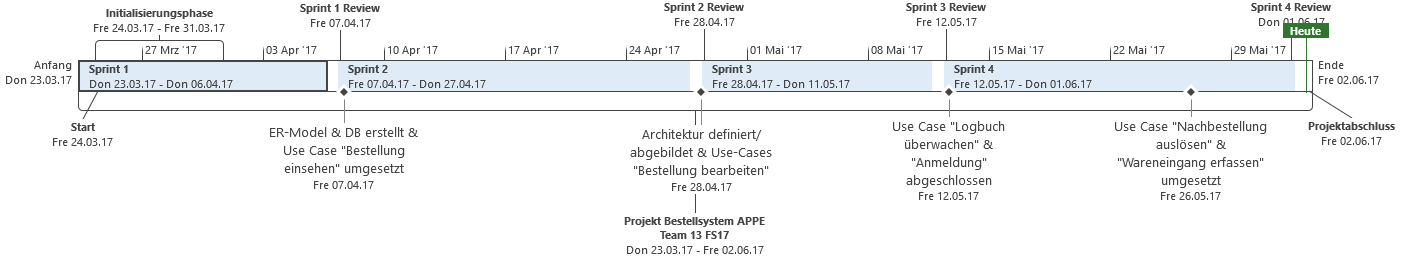
\includegraphics[width=1.0\textwidth]{Images/GroberTerminplan.png}
\label{fig:title}
\end{figure}
Das Projekt wird vom 23.03.2017 bis am 02.06.2017 durchgeführt. Zur regelmässigen Kontrolle \↨& Planung wird die Projektdauer in vier Entwicklungssprints unterteilt. Auf dem Weg zur finalen Version werden ebenfalls vier Meilensteine wie folgt gesetzt:
\begin{enumerate}
\item Meilenstein 1 \textit{ER-Modell \& DB erstellt \& Use Case 'Bestellung einsehen' umgesetzt}\\
Neben den Initialisierungsaufgaben wie Erstellung PMP \& SysSpec und initiale Anforderungsaufnahme liegt die DB anhand des vorgängig erstellten ER-Modell vor. Weiter ist der erste Use Case 'Bestellung einsehen' umgesetzt
\item Meilenstein 2 \textit{Architektur definiert \& Use Case 'Bestellung bearbeiten' umgesetzt}\\
Neben der Layer- \& Tierarchitektur, Komponentenschnitt ist der Use Case 'Bestellung bearbeiten' vollständig umgesetzt. 
\item Meilenstein 3 \textit{Use Case 'Nachbestellung' \& 'Anmeldung' umgesetzt} \\
Alle Use Cases bis auf 'Logbuch überwachen' sind umgesetzt. Erste Integrations- \& Systemtests sind ausgeführt.
\item Meilenstein 4 \textit{Use Case 'Logbuch überwachen' \& Dokumentation abgeschlossen}\\
Neben dem letzten Use Case 'Logbuch überwachen' werden alle Integrations- \& Systemtests durchgeführt. Abschliessend liegen die SysSpec und der PMP vor.
\end{enumerate}

\subsubsection{Projektkontrolle}
In der Projektkontrolle sollen Abweichungen zwischen SOLL- und IST-Zustand aufgedeckt werden. Der Zustand bezieht sich auf den Projektfortschritt. In jedem Sprint werden Arbeitspakete definiert und mit einem bestimmten Aufwand (in Stunden) versehen
\subsubsection{Risikomanagement}

\subsubsection{Projektabschluss}
% !TEX root = Dokumentation_PMP.tex
\section{Projektunterstützung}
Im Zentrum stehen hier Werkzeuge, welche das Team in ihrer Arbeit unterstützen sollen.
Ausserdem werden hier auch das Konfigurations-Management beschrieben, welche pro Sprint vorliegen.
\subsection{Tools für Entwicklung, Test \& Abnahme}
Im Rahmen des Moduls werden folgende Tools verwendet.
\begin{table}[H]
\begin{tabular}{ | p{0.30\textwidth} | p{0.70\textwidth} | }
\hline \rowcolor{gray!50}
%Titelzeile
	\textbf{Zweck} 		 &
	\textbf{Tool}
	\\	\hline
%Zeile
	Scrum-Tool 	&
	ScrumDo (Online)
	\\  \hline	%Untere Abgrenzung
%Zeile
	ERM-/ERD-Designer 		&
	MySQL Workbench v.6.3
	\\  \hline	%Untere Abgrenzung
%Zeile
	UML-Designer 		&
	Dia v0.97.2 \& MS Visio 2016
	\\  \hline	%Untere Abgrenzung
%Zeile
	Entwicklungsumgebung 		&
	Eclipse Neon 3
	\\  \hline	%Untere Abgrenzung
%Zeile
	Sourcecode Verwaltung 		&
	GitLab CE 8.14.2
	\\  \hline	%Untere Abgrenzung
%Zeile
	Sourcecode Style 		&
	CheckStyle / PMD / JaCoCo (Coverage)
	\\  \hline	%Untere Abgrenzung
%Zeile
	Buildserver 		&
	Maven, Jenkins v.1.558
	\\  \hline	%Untere Abgrenzung
%Zeile
	Test 		&
	JUnit / manuelle Integrations-Tests
	\\  \hline	%Untere Abgrenzung
%Zeile
	Dokumentation 		&
	\LaTeX  on GitHub
	\\  \hline	%Untere Abgrenzung
\end{tabular}
\label{tab:tooling}
\caption{Tools}
\end{table}


\subsection{Konfigurationsmanagement}
Jede Komponente wird versioniert. Sie kann nur mit definierten Versionen anderer Komponenten im Verbund korrekt zusammenarbeiten. Daher werden hier die Komponentenversionen pro Sprint (shippable Software) aufgelistet. Die Tests basieren auf diesen Versionen.
\subsubsection{Softwarekomponenten}
\begin{table}[H]
\begin{tabular}{ | p{0.20\textwidth} | p{0.10\textwidth} | p{0.10\textwidth} | p{0.10\textwidth} | p{0.10\textwidth} | }
\hline \rowcolor{gray!50}
%Titelzeile
	\textbf{Artefakt} 		 &
	\textbf{Sprint 1}	 	 &
	\textbf{Sprint 2}	 	 &
	\textbf{Sprint 3}		 &
	\textbf{Sprint 4}
	\\	\hline
%Zeile
	fbs\_business 	&
	v0.1.2 			&
	v0.2.1 			&
	v0.3.5 			&
	v1.0.0
	\\  \hline	%Untere Abgrenzung
%Zeile
	fbs\_client 		&
	v0.1.5 			&
	v0.2.0 			&
	v0.3.1 			&
	v1.0.0
	\\  \hline	%Untere Abgrenzung
%Zeile
	fbs\_data 		&
	v0.1.3 			&
	v0.2.6 			&
	v0.3.2 			&
	v1.0.0
	\\  \hline	%Untere Abgrenzung
%Zeile
	fbs\_model 		&
	v0.1.1 			&
	v0.2.0 			&
	v0.3.0 			&
	v1.0.0
	\\  \hline	%Untere Abgrenzung
\end{tabular}
\label{tab:config_sw}
\caption{Softwarekomponenten Konfigurationsmanagement}
\end{table}

\subsubsection{Dokumentation}
\begin{table}[H]
\begin{tabular}{ | p{0.30\textwidth} | p{0.10\textwidth} | p{0.10\textwidth} | p{0.10\textwidth} | p{0.10\textwidth} | }
\hline \rowcolor{gray!50}
%Titelzeile
	\textbf{Dokument} 		&
	\textbf{Sprint 1}	 	&
	\textbf{Sprint 2}	 	&
	\textbf{Sprint 3}		&
	\textbf{Sprint 4}
	\\	\hline
%Zeile
	Projektmanagementplan 	&
	v0.1 					&
	v0.3 					&
	v0.5 					&
	v1.0
	\\  \hline	%Untere Abgrenzung
%Zeile
	Systemspezifikation 	&
	v0.1 					&
	v0.1 					&
	v0.2 					&
	v1.0
	\\  \hline	%Untere Abgrenzung
\end{tabular}
\label{tab:config_dok}
\caption{Dokumentation Konfigurationsmanagement}
\end{table}


% !TEX root = Dokumentation_PMP.tex
\section{Testplan}
\subsection{Testdesign \& Abläufe}
Dieses Kapitel hält Integrations- und Systemtests fest. \\
Unittests wurden womöglich aktiv eingesetzt, wenn die zeitlichen Aufwände nicht zu hoch sind. Die Entscheidung obliegt jedem einzelnen Entwickler. Es wurde im Team entschieden, dass GUI-Elemente /-Klassen bewusst nicht mittels Unit-Tests abgedeckt werden. \\
Das Team strebt daher keine hohe Codeabdeckung an und setzt als Schwellwert > 30\% Codeabdeckung summarisch über alle Projekte gem. Jenkins-Report. \\
Der Unterschied beider Testarten ist folgender: Integrationstest sind teilautomatisiert mittels JUnit. Diese Tests können in der Entwicklungsumgebung nach dem Setup der Testumgebung gestartet werden. Wohingegen Systemtests vollständig manuell sind.
\subsection{Integrationstests}
% !TEX root = Dokumentation.tex
\subsubsection{Integrationstest 1}
\begin{table}[H]
\begin{tabular}{ | p{0.22\textwidth} | p{0.68\textwidth} |} \hline
\rowcolor{gray!50}
%Titelzeile
	\textbf{ID}          &
	\begin{tabular}{l}
		\textbf{I1}
	\end{tabular}
	\\ \hline
%Zeile
	\textbf{Bezeichnung}			 &
	\begin{tabular}{l}
		Applikation \glqq{}Filialbestelsystem\grqq{} kann gestartet werden.
	\end{tabular}
\\ \hline
%Zeile
	\textbf{Beschreibung}   		 &
	\begin{tabular}{l}
		Die Applikation kann gestartet werden.
	\end{tabular}
\\ \hline
%Zeile
	\textbf{Akteure}              & 
	\begin{tabular}{l}
		Nutzer
	\end{tabular}
\\ \hline
%Zeile
	\textbf{Vorbedingungen}       &
	\begin{tabular}{l}
		keine
	\end{tabular}		
\\ \hline
%Zeile
	\textbf{Ergebnis}             &        
	\begin{tabular}{l}
		Integrationstest werden fehlerfrei abgeschlossen. \\
		Die Applikation ist erfolgreich gestartet. \\
		Die Anmelde-Maske wird gestartet. \\
	\end{tabular}
\\ \hline
%Zeile
	\textbf{Ergebnis bei Fehler}  &
	\begin{tabular}{l}
		- Exception\\
		- Unit Test failed
	\end{tabular}
\\ \hline
%Zeile
	\textbf{Ablauf}				 &
	\begin{tabular}{l}
		1. Applikation starten\\
		2. Ergebnis prüfen
	\end{tabular}
\\ \hline
	\textbf{Testdaten}            &
	\begin{tabular}{l}
		Keine benötigt.
	\end{tabular}
\\ \hline	%Untere Abgrenzung
\end{tabular}
\end{table}
% !TEX root = Dokumentation.tex
\subsubsection{Integrationstest 2}
\begin{table}[H]
\begin{tabular}{ | p{0.22\textwidth} | p{0.68\textwidth} |} \hline
\rowcolor{gray!50}
%Titelzeile
	\textbf{ID}          &
	\begin{tabular}{l}
		\textbf{I2}
	\end{tabular}
	\\ \hline
%Zeile
	\textbf{Bezeichnung}			 &
	\begin{tabular}{l}
		Anmeldung an Applikation funktioniert.
	\end{tabular}
\\ \hline
%Zeile
	\textbf{Beschreibung}   		 &
	\begin{tabular}{l}
		Die Anmeldung mit Username und Passwort funktioniert\\
		an der Applikation.
	\end{tabular}
\\ \hline
%Zeile
	\textbf{Akteure}              & 
	\begin{tabular}{l}
		Benutzer
	\end{tabular}
\\ \hline
%Zeile
	\textbf{Vorbedingungen}       &
	\begin{tabular}{l}
		Applikation erfolgreich gestartet
	\end{tabular}		
\\ \hline
%Zeile
	\textbf{Ergebnis}             &        
	\begin{tabular}{l}
		Anmeldung erfolgreich\\
Benutzeransicht nach Benutzergruppe erscheint
	\end{tabular}
\\ \hline
%Zeile
	\textbf{Ergebnis bei Fehler}  &
	\begin{tabular}{l}
		- Fehlermeldung erscheint\\
	\end{tabular}
\\ \hline
%Zeile
	\textbf{Ablauf}				 &
	\begin{tabular}{l}
		1. Username eingeben\\
		2. Passwort eingeben\\
		3. Anmeldung bestätigen
	\end{tabular}
\\ \hline
	\textbf{Testdaten}            &
	\begin{tabular}{l}
		Username, Passwort und Gruppenzugehörigkeit.
	\end{tabular}
\\ \hline	%Untere Abgrenzung
\end{tabular}
\end{table}
% !TEX root = Dokumentation_PMP.tex
\subsubsection{Integrationstest 3 - Erfassung Wareneingang}
\begin{table}[H]
\begin{tabular}{ | p{0.22\textwidth} | p{0.68\textwidth} |} \hline
\rowcolor{gray!50}
%Titelzeile
	\textbf{ID}						&
	\begin{tabular}{l}
		\textbf{I3}
	\end{tabular}
	\\ \hline
%Zeile
	\textbf{Bezeichnung}			&
	\begin{tabular}{l}
		Wareneingang kann erfasst werden.
	\end{tabular}
\\ \hline
%Zeile
	\textbf{Beschreibung}			&
	\begin{tabular}{l}
		Die Erfassung von Lieferungen ans Filiallager kann erfasst werden.
	\end{tabular}
\\ \hline
%Zeile
	\textbf{Akteure}				& 
	\begin{tabular}{l}
		Datentypist
	\end{tabular}
\\ \hline
%Zeile
	\textbf{Vorbedingungen}			&
	\begin{tabular}{l}
		Applikation erfolgreich gestartet\\
Anmeldung erfolgreich\\
Benutzergruppe Datentypist zugewiesen
	\end{tabular}		
\\ \hline
%Zeile
	\textbf{Ergebnis}				&        
	\begin{tabular}{l}
		Bestätigung der erfassten Lieferung.
	\end{tabular}
\\ \hline
%Zeile
	\textbf{Ergebnis bei Fehler}	&
	\begin{tabular}{l}
		- Fehlermeldung erscheint
	\end{tabular}
\\ \hline
%Zeile
	\textbf{Ablauf}					&
	\begin{tabular}{l}
		1. Formular ausfüllen\\
		2. Formular absenden\\
		3. Bestätigung erhalten
	\end{tabular}
\\ \hline
	\textbf{Testdaten}				&
	\begin{tabular}{l}
		Test-Lieferung.
	\end{tabular}
\\ \hline	%Untere Abgrenzung
\end{tabular}
\end{table}
% !TEX root = Dokumentation.tex
\subsubsection{Integrationstest 5}
\begin{table}[H]
\begin{tabular}{ | p{0.22\textwidth} | p{0.68\textwidth} |} \hline
\rowcolor{gray!50}
%Titelzeile
	\textbf{ID}						&
	\begin{tabular}{l}
		\textbf{I5}
	\end{tabular}
	\\ \hline
%Zeile
	\textbf{Bezeichnung}			&
	\begin{tabular}{l}
		Nachbestellung einsehen.
	\end{tabular}
\\ \hline
%Zeile
	\textbf{Beschreibung}			&
	\begin{tabular}{l}
		Die offenen Nachbestellungen am Zentrallager können eingesehen\\
werden.
	\end{tabular}
\\ \hline
%Zeile
	\textbf{Akteure}				& 
	\begin{tabular}{l}
		Filialleiter
	\end{tabular}
\\ \hline
%Zeile
	\textbf{Vorbedingungen}			&
	\begin{tabular}{l}
		Nachbestellung offen.\\
		Erfolgreich an System angemeldet.\\
		Benutzergruppe zugewiesen.
	\end{tabular}		
\\ \hline
%Zeile
	\textbf{Ergebnis}				&
	\begin{tabular}{l}
		Nachbestellung wird angezeigt
	\end{tabular}
\\ \hline
%Zeile
	\textbf{Ergebnis bei Fehler}	&
	\begin{tabular}{l}
		- Fehlermeldung erscheint
	\end{tabular}
\\ \hline
%Zeile
	\textbf{Ablauf}					&
	\begin{tabular}{l}
		1. Nachbestellung ansehen
	\end{tabular}
\\ \hline
	\textbf{Testdaten}				&
	\begin{tabular}{l}
		Vorhandene Nachbestellung.
	\end{tabular}
\\ \hline	%Untere Abgrenzung
\end{tabular}
\end{table}
% !TEX root = Dokumentation.tex
\subsubsection{Integrationstest 6 - Bestellung einsehen}
\begin{table}[H]
\begin{tabular}{ | p{0.22\textwidth} | p{0.68\textwidth} |} \hline
\rowcolor{gray!50}
%Titelzeile
	\textbf{ID}						&
	\begin{tabular}{l}
		\textbf{I6}
	\end{tabular}
	\\ \hline
%Zeile
	\textbf{Bezeichnung}			&
	\begin{tabular}{l}
		Bestellung einsehen
	\end{tabular}
\\ \hline
%Zeile
	\textbf{Beschreibung}			&
	\begin{tabular}{l}
		Bestellungen können eingesehen
werden.
	\end{tabular}
\\ \hline
%Zeile
	\textbf{Akteure}				&
	\begin{tabular}{l}
		Filialleiter, Verkaufspersonal.
	\end{tabular}
\\ \hline
%Zeile
	\textbf{Vorbedingungen}			&
	\begin{tabular}{l}
		Offene Bestellung vorhanden.\\
		Erfolgreich an System angemeldet.\\
		Benutzergruppe zugewiesen.
	\end{tabular}		
\\ \hline
%Zeile
	\textbf{Ergebnis}				&
	\begin{tabular}{l}
		Bestellung wird angezeigt
	\end{tabular}
\\ \hline
%Zeile
	\textbf{Ergebnis bei Fehler}	&
	\begin{tabular}{l}
		- Fehlermeldung erscheint
	\end{tabular}
\\ \hline
%Zeile
	\textbf{Ablauf}					&
	\begin{tabular}{l}
		1. Bestellungen ansehen
	\end{tabular}
\\ \hline
	\textbf{Testdaten}				&
	\begin{tabular}{l}
		Test-Bestellung.
	\end{tabular}
\\ \hline	%Untere Abgrenzung
\end{tabular}
\end{table}
% !TEX root = Dokumentation_PMP.tex
\subsubsection{Integrationstest 6 - Bestellung annullieren}
\begin{table}[H]
\begin{tabular}{ | p{0.22\textwidth} | p{0.68\textwidth} |} \hline
\rowcolor{gray!50}
%Titelzeile
	\textbf{ID}						&
	\begin{tabular}{l}
		\textbf{I7}
	\end{tabular}
	\\ \hline
%Zeile
	\textbf{Bezeichnung}			&
	\begin{tabular}{l}
		Bestellung annullieren.
	\end{tabular}
\\ \hline
%Zeile
	\textbf{Zugehörige Userstory}			 &
	\begin{tabular}{l}
		Bestellung annulieren (I8-4)
	\end{tabular}
\\ \hline
%Zeile
	\textbf{Beschreibung}			&
	\begin{tabular}{l}
		Eine Bestellung kann annulliert werden.
	\end{tabular}
\\ \hline
%Zeile
	\textbf{Akteure}				&
	\begin{tabular}{l}
		Filialleiter, Verkaufspersonal.
	\end{tabular}
\\ \hline
%Zeile
	\textbf{Vorbedingungen}			&
	\begin{tabular}{l}
		Offene Bestellung vorhanden.\\
		Erfolgreich an System angemeldet.\\
		Benutzergruppe zugewiesen.
	\end{tabular}		
\\ \hline
%Zeile
	\textbf{Ergebnis}				&
	\begin{tabular}{l}
		Bestellung annulliert.\\
		Rechnungswesen notifiziert.
	\end{tabular}
\\ \hline
%Zeile
	\textbf{Ergebnis bei Fehler}	&
	\begin{tabular}{l}
		- Fehlermeldung erscheint
	\end{tabular}
\\ \hline
%Zeile
	\textbf{Ablauf}					&
	\begin{tabular}{l}
		1. Bestellung öffnen\\
		2. Bestellung annullieren.
		3. Rechnungswesen notifizieren.\\
		4. Filiallager notifizieren.\\
		5. Bestätigung.
	\end{tabular}
\\ \hline
	\textbf{Testdaten}				&
	\begin{tabular}{l}
		Test-Bestellung.
	\end{tabular}
\\ \hline	%Untere Abgrenzung
\end{tabular}
\end{table}
% !TEX root = Dokumentation.tex
\subsubsection{Integrationstest 8 - Bestellung editieren}
\begin{table}[H]
\begin{tabular}{ | p{0.22\textwidth} | p{0.68\textwidth} |} \hline
\rowcolor{gray!50}
%Titelzeile
	\textbf{ID}						&
	\begin{tabular}{l}
		\textbf{I7}
	\end{tabular}
	\\ \hline
%Zeile
	\textbf{Bezeichnung}			&
	\begin{tabular}{l}
		Bestellung editieren.
	\end{tabular}
\\ \hline
%Zeile
	\textbf{Beschreibung}			&
	\begin{tabular}{l}
		Eine Bestellung kann editiert werden.
	\end{tabular}
\\ \hline
%Zeile
	\textbf{Akteure}				&
	\begin{tabular}{l}
		Filialleiter, Verkaufspersonal.
	\end{tabular}
\\ \hline
%Zeile
	\textbf{Vorbedingungen}			&
	\begin{tabular}{l}
		Offene Bestellung vorhanden.\\
		Erfolgreich an System angemeldet.\\
		Benutzergruppe zugewiesen.
	\end{tabular}		
\\ \hline
%Zeile
	\textbf{Ergebnis}				&
	\begin{tabular}{l}
		Bestellung editiert.\\
		Rechnungswesen notifiziert.
	\end{tabular}
\\ \hline
%Zeile
	\textbf{Ergebnis bei Fehler}	&
	\begin{tabular}{l}
		- Fehlermeldung erscheint
	\end{tabular}
\\ \hline
%Zeile
	\textbf{Ablauf}					&
	\begin{tabular}{l}
		1. Bestellung öffnen.\\
		2. Bestellung editieren und bestätigen.
		3. Rechnungswesen notifizieren.\\
		4. Filiallager notifizieren.\\
		5. Bestätigung.
	\end{tabular}
\\ \hline
	\textbf{Testdaten}				&
	\begin{tabular}{l}
		Test-Bestellung.
	\end{tabular}
\\ \hline	%Untere Abgrenzung
\end{tabular}
\end{table}
% !TEX root = Dokumentation_PMP.tex
\subsubsection{Integrationstest 8 - Bestellung erfassen}
\begin{table}[H]
\begin{tabular}{ | p{0.22\textwidth} | p{0.68\textwidth} |} \hline
\rowcolor{gray!50}
%Titelzeile
	\textbf{ID}								&
	\begin{tabular}{l}
		\textbf{I7}
	\end{tabular}
	\\ \hline
%Zeile
	\textbf{Bezeichnung}					&
	\begin{tabular}{l}
		Bestellung erfassen.
	\end{tabular}
\\ \hline
%Zeile
	\textbf{Zugehörige Userstory}			 &
	\begin{tabular}{l}
		Bestellung erfassen (I8-1)
	\end{tabular}
\\ \hline
%Zeile
	\textbf{Beschreibung}					&
	\begin{tabular}{l}
		Eine Bestellung kann erfasst
werden.
	\end{tabular}
\\ \hline
%Zeile
	\textbf{Akteure}						&
	\begin{tabular}{l}
		Filialleiter, Verkaufspersonal.
	\end{tabular}
\\ \hline
%Zeile
	\textbf{Vorbedingungen}					&
	\begin{tabular}{l}
		Erfolgreich an System angemeldet.\\
		Benutzergruppe zugewiesen.\\
		Für Testkunde keine offenen Mahnungen vorhanden.
	\end{tabular}		
\\ \hline
%Zeile
	\textbf{Ergebnis}						&
	\begin{tabular}{l}
		Bestellung erfasst.\\
		Rechnungswesen notifiziert.\\
		Filiallager notifiziert.
	\end{tabular}
\\ \hline
%Zeile
	\textbf{Ergebnis bei Fehler}			&
	\begin{tabular}{l}
		- Fehlermeldung erscheint
	\end{tabular}
\\ \hline
%Zeile
	\textbf{Ablauf}							&
	\begin{tabular}{l}
		1. Bestellung erfassen und bestätigen.
		3. Rechnungswesen notifizieren.\\
		4. Filiallager notifizieren.\\
		5. Bestätigung.
	\end{tabular}
\\ \hline
	\textbf{Testdaten}						&
	\begin{tabular}{l}
		Testkunde.
	\end{tabular}
\\ \hline	%Untere Abgrenzung
\end{tabular}
\end{table}
% systemtests
\clearpage
\subsection{Systemtests}
\subsubsection{Vorbereitung}
Als generelle Vorbedingung gilt jeweils ein komplett installiertes System. Zur Installation benötigt man die Installationspakete, welche nach einem Build unter ‚build lib‘ zu finden sind. Bevor mit den Systemtests gestartet wird, sollten alle Unit- sowie Integrationstests erfolgreich durchgeführt worden sein.
% !TEX root = Dokumentation.tex
\subsubsection{Systemtest 1}
\begin{table}[H]
\begin{tabular}{ | p{0.22\textwidth} | p{0.68\textwidth} |} \hline
\rowcolor{gray!50}
%Titelzeile
	\textbf{ID}          &
	\begin{tabular}{l}
		\textbf{S1}
	\end{tabular}
	\\ \hline
%Zeile
	\textbf{Bezeichnung}			 &
	\begin{tabular}{l}
		Wareneingang erfassen.
	\end{tabular}
\\ \hline
%Zeile
	\textbf{Beschreibung}   		 &
	\begin{tabular}{l}
		Der Wareneingang wird im Filialbestellsystem erfasst und ist in der\\
Datenbank persistiert.
	\end{tabular}
\\ \hline
%Zeile
	\textbf{Akteure}              & 
	\begin{tabular}{l}
		Datentypist
	\end{tabular}
\\ \hline
%Zeile
	\textbf{Vorbedingungen}       &
	\begin{tabular}{l}
		Erfolgreich als Datentypist im System angemeldet.
	\end{tabular}		
\\ \hline
%Zeile
	\textbf{Ergebnis}             &        
	\begin{tabular}{l}
		Die erfassten Wareneingänge sind in der Datenbank persistiert.
	\end{tabular}
\\ \hline
%Zeile
	\textbf{Ergebnis bei Fehler}  &
	\begin{tabular}{l}
		- Fehlermeldung
	\end{tabular}
\\ \hline
%Zeile
	\textbf{Ablauf}				 &
	\begin{tabular}{l}
		1. Anmeldung als Datentypist\\
		2. Erfassung starten\\
		3. Persistierung\\
		4. Lagerbestand kontrollieren
	\end{tabular}
\\ \hline	%Untere Abgrenzung
\end{tabular}
\end{table}
% !TEX root = Dokumentation_PMP.tex
\subsubsection{Systemtest 1 - Automatische Nachbestellung}
\begin{table}[H]
\begin{tabular}{ | p{0.22\textwidth} | p{0.68\textwidth} |} \hline
\rowcolor{gray!50}
%Titelzeile
	\textbf{ID}          &
	\begin{tabular}{l}
		\textbf{S2}
	\end{tabular}
	\\ \hline
%Zeile
	\textbf{Bezeichnung}			 &
	\begin{tabular}{l}
		Automatische Nachbestellung auslösen.
	\end{tabular}
\\ \hline
%Zeile
	\textbf{Zugehörige Userstory}			 &
	\begin{tabular}{l}
		Nachbestellung auslösen (I8-7)
	\end{tabular}
\\ \hline
%Zeile
	\textbf{Beschreibung}   		 &
	\begin{tabular}{l}
		Das Filialbestellsystem löst automatisch eine Nachbestellung aus, wenn\\
ein definierter Lagerbestand unterschritten wird.
	\end{tabular}
\\ \hline
%Zeile
	\textbf{Akteure}              & 
	\begin{tabular}{l}
		Filialbestellsystem, Filialleiter, Filialverwalter
	\end{tabular}
\\ \hline
%Zeile
	\textbf{Vorbedingungen}       &
	\begin{tabular}{l}
		Lagerbestand unterschreitet Mindestlagerbestand.
	\end{tabular}		
\\ \hline
%Zeile
	\textbf{Ergebnis}             &        
	\begin{tabular}{l}
		Nachbestellung ausgelöst\\
		Filialleiter kann Nachbestellung einsehen\\
		Filialverwalter sieht Logeintrag.
	\end{tabular}
\\ \hline
%Zeile
	\textbf{Ergebnis bei Fehler}  &
	\begin{tabular}{l}
		- nfo an Filialleiter
	\end{tabular}
\\ \hline
%Zeile
	\textbf{Ablauf}				 &
	\begin{tabular}{l}
		1. Lagerbestand unterschreiten\\
		2. Nachbestellung auslösen\\
		3. Log-Eintrag erstellen\\
		4. Nachbestellung prüfen (Filialverwalter)
	\end{tabular}
\\ \hline	%Untere Abgrenzung
\end{tabular}
\end{table}
% !TEX root = Dokumentation.tex
\subsubsection{Systemtest 3}
\begin{table}[H]
\begin{tabular}{ | p{0.22\textwidth} | p{0.68\textwidth} |} \hline
\rowcolor{gray!50}
%Titelzeile
	\textbf{ID}          &
	\begin{tabular}{l}
		\textbf{S3}
	\end{tabular}
	\\ \hline
%Zeile
	\textbf{Bezeichnung}			 &
	\begin{tabular}{l}
		Bestellung bearbeiten.
	\end{tabular}
\\ \hline
%Zeile
	\textbf{Beschreibung}   		 &
	\begin{tabular}{l}
		Bestellungen können im System bearbeitet werden.
	\end{tabular}
\\ \hline
%Zeile
	\textbf{Akteure}              & 
	\begin{tabular}{l}
		Verkaufspersonal (Filialleiter)
	\end{tabular}
\\ \hline
%Zeile
	\textbf{Vorbedingungen}       &
	\begin{tabular}{l}
		Anmeldung als Verkaufspersonal (Filialleiter) am System.
	\end{tabular}		
\\ \hline
%Zeile
	\textbf{Ergebnis}             &        
	\begin{tabular}{l}
		Teil-Ergebnisse:\\
		 1. Bestellung kann erfasst werden.\\
		 2. Bestellung kann bearbeitet werden.\\
		 3. Bestellung kann annulliert werden.\\
		 4. Bestellung kann eingesehen werden.
		Lagerbestand aktualisiert.\\
		Rechnungswesen informiert.\\
		Bestellbestätigung ausgelöst.\\
	\end{tabular}
\\ \hline
%Zeile
	\textbf{Ergebnis bei Fehler}  &
	\begin{tabular}{l}
		- Fehlermeldung
	\end{tabular}
\\ \hline
%Zeile
	\textbf{Ablauf}				 &
	\begin{tabular}{l}
		1. Bestellung erfassen\\
		2. Bestellung ansehen.\\
		3. Bestellung bearbeiten.\\
		4. Bestellung ansehen.\\
		5. Bestellung annullieren.\\
	\end{tabular}
\\ \hline	%Untere Abgrenzung
\end{tabular}
\end{table}

\section{Anhänge}
\end{document}
